\documentclass[12pt,a4paper,oneside]{report}

\usepackage[margin=1in]{geometry}
\usepackage[T1]{fontenc}
\usepackage[utf8]{inputenc}
\usepackage{newtxtext,newtxmath}
\usepackage{setspace}
\usepackage{graphicx}
\usepackage{booktabs}
\usepackage{array}
\usepackage{multirow}
\usepackage{longtable}
\usepackage{tabularx}
\usepackage{amsmath,amssymb}
\usepackage{algorithm}
\usepackage{algorithmic}
\usepackage{xcolor}
\usepackage{tikz}
\usetikzlibrary{arrows.meta,positioning,shapes.geometric,fit,calc}
\usepackage{caption}
\usepackage{subcaption}
\usepackage{hyperref}
\usepackage{cite}
\usepackage{float}
\usepackage{listings}
\usepackage{enumitem}

\hypersetup{colorlinks=true, linkcolor=black, citecolor=blue, urlcolor=blue}
\graphicspath{{figures/}{../results/}}
\onehalfspacing
\setlength{\parskip}{0.35em}
\setlength{\parindent}{1.2em}

\newcommand{\thesistitle}{Machine Learning-Based Protein Biomarker Identification for Chronic Kidney Disease Using Single-Cell RNA Sequencing Data}
\newcommand{\studentname}{Student Name}
\newcommand{\studentid}{Student ID}
\newcommand{\supervisor}{Supervisor Name}
\newcommand{\department}{Department of Computer Science and Engineering}
\newcommand{\university}{University Name}

\begin{document}
\pagenumbering{roman}
\begin{titlepage}
\centering
{\Large \university\\[0.3cm]}
{\large \department\\[1.5cm]}
{\bfseries\LARGE \thesistitle \par}
\vspace{1.5cm}
{\large A thesis submitted in partial fulfillment of the requirements for the degree of\\[0.2cm]
Bachelor of Science in Computer Science and Engineering\par}
\vfill
\begin{tabular}{rl}
Submitted by: & \studentname \\
Student ID: & \studentid \\
Supervisor: & \supervisor \\
\end{tabular}
\vfill
{\large May 2026}
\end{titlepage}

\chapter*{Approval Page}
This thesis titled ``\thesistitle'' submitted by \studentname, Student ID \studentid, has been accepted as satisfactory in partial fulfillment of the requirements for the degree of Bachelor of Science in Computer Science and Engineering.

\vspace{1.5cm}
\begin{tabular}{p{0.45\textwidth}p{0.45\textwidth}}
\rule{0.42\textwidth}{0.4pt} & \rule{0.42\textwidth}{0.4pt}\\
Supervisor & Head of Department\\[1.2cm]
\rule{0.42\textwidth}{0.4pt} & \rule{0.42\textwidth}{0.4pt}\\
Examiner 1 & Examiner 2\\
\end{tabular}
\clearpage

\chapter*{Declaration}
I declare that this thesis is my original work and that it has not been submitted elsewhere for any degree or diploma. All sources of information used in this study have been acknowledged through appropriate IEEE-style citations.

\vspace{1.2cm}
\noindent\rule{0.4\textwidth}{0.4pt}\\
\studentname
\clearpage

\chapter*{Abstract}
Chronic kidney disease (CKD) is a progressive renal disorder associated with nephron loss, inflammation, extracellular matrix deposition, and irreversible decline in kidney function. Acute kidney injury (AKI) may resolve after transient damage, but incomplete repair can increase the risk of CKD progression. This thesis presents a machine learning-based computational framework for identifying candidate protein biomarker genes associated with AKI, CKD, and CKD progression using single-cell RNA sequencing data from the GSE183276 Human Kidney Healthy and Injury Cell Atlas. Raw count data were processed using quality control filtering, library-size normalization, log transformation, and highly variable gene selection. The final feature matrix consisted of the top 3000 highly variable genes ranked by variance, with single cells as samples and \texttt{condition.l1} labels representing reference, AKI, and CKD conditions. Random Forest classifiers were trained using balanced class weights, and feature importance scores were combined with absolute expression differences to prioritize biomarkers. Pairwise analyses were performed for AKI versus reference, CKD versus reference, and CKD versus AKI. The results emphasize biologically meaningful injury and fibrosis-associated genes, including \textit{HAVCR1}, \textit{LCN2}, \textit{COL1A1}, \textit{FN1}, and \textit{SERPINE1}. The proposed workflow demonstrates how interpretable machine learning and single-cell transcriptomics can support biomarker discovery for kidney disease.

\textbf{Keywords:} chronic kidney disease, acute kidney injury, single-cell RNA sequencing, Random Forest, biomarker discovery, highly variable genes, kidney fibrosis.
\clearpage

\chapter*{Acknowledgement}
I express sincere gratitude to my supervisor for guidance, feedback, and encouragement throughout this thesis. I also acknowledge the researchers who generated and made publicly available the GSE183276 Human Kidney Healthy and Injury Cell Atlas dataset. Finally, I thank my department, teachers, family, and peers for their support during the completion of this work.
\clearpage

\tableofcontents
\listoffigures
\listoftables
\clearpage
\pagenumbering{arabic}

\chapter{Introduction}
\section{Background}
Kidney disease represents a major global health challenge because renal dysfunction is often detected after substantial tissue injury has already occurred. Chronic kidney disease (CKD) is defined by persistent abnormalities in kidney structure or function and is associated with increased risk of cardiovascular disease, kidney failure, and mortality \cite{kdigo2024ckd}. Acute kidney injury (AKI) is a rapid decline in kidney function caused by ischemic, toxic, inflammatory, or obstructive insults. Although AKI is clinically distinct from CKD, experimental and clinical evidence suggests that unresolved AKI can contribute to CKD through maladaptive repair, persistent inflammation, capillary rarefaction, and fibrosis \cite{chawla2014aki_ckd}.

Traditional bulk transcriptomics averages gene expression across mixed cell populations. In contrast, single-cell RNA sequencing (scRNA-seq) measures transcript abundance at cellular resolution, allowing disease-associated signals to be examined in heterogeneous kidney tissue \cite{liao2020singlecell}. This is especially important for the kidney because its function depends on specialized epithelial, endothelial, stromal, and immune cell populations.

\section{Problem Statement}
Reliable biomarkers are needed to distinguish healthy reference kidney tissue, AKI, CKD, and potential CKD progression states. Existing clinical markers such as serum creatinine are delayed and non-specific. Transcriptomic biomarker discovery can identify genes associated with injury, fibrosis, and disease progression, but scRNA-seq data are high-dimensional, sparse, noisy, and class-imbalanced. Therefore, computational approaches must combine biological preprocessing with interpretable machine learning.

\section{Objectives}
The objectives of this thesis are:
\begin{enumerate}[label=\arabic*.]
\item To preprocess the GSE183276 scRNA-seq dataset using QC filtering, normalization, log transformation, and highly variable gene selection.
\item To train Random Forest classifiers for disease-state prediction using the top 3000 highly variable genes.
\item To identify candidate biomarkers for AKI, CKD, and CKD progression through pairwise comparisons.
\item To rank biomarkers using a combined score based on Random Forest importance and expression difference.
\item To interpret top genes in relation to tubular injury, inflammation, extracellular matrix remodeling, and fibrosis.
\end{enumerate}

\section{Contributions}
This work contributes a reproducible BSc-level bioinformatics and machine learning framework for kidney disease biomarker discovery. The framework integrates single-cell preprocessing, feature selection, Random Forest classification, pairwise biomarker prioritization, and thesis-ready visualization.

\section{Thesis Organization}
Chapter 2 reviews related literature. Chapter 3 describes materials and methods. Chapter 4 explains dataset preparation and preprocessing. Chapter 5 presents the machine learning methodology. Chapter 6 discusses results. Chapter 7 interprets candidate biomarkers. Chapter 8 concludes the thesis and outlines future work.

\chapter{Literature Review}
\section{CKD Biomarkers}
CKD biomarker research has focused on markers of filtration, tubular damage, inflammation, and fibrosis. Fibrosis is a central pathological feature of CKD and involves extracellular matrix accumulation, myofibroblast activation, and altered epithelial-stromal communication \cite{liu2011fibrosis}. Genes such as \textit{COL1A1} and \textit{FN1} are frequently associated with matrix deposition and remodeling. \textit{SERPINE1}, which encodes plasminogen activator inhibitor-1, has been linked with profibrotic signaling and impaired extracellular matrix turnover.

\section{AKI Biomarkers}
AKI biomarkers aim to detect renal injury before conventional clinical markers become abnormal. \textit{HAVCR1}, encoding kidney injury molecule-1 (KIM-1), is widely studied as a proximal tubule injury marker. \textit{LCN2}, encoding neutrophil gelatinase-associated lipocalin (NGAL), is associated with tubular stress, inflammation, and early kidney injury \cite{devarajan2008ngal}. These markers provide biological context for transcriptomic injury signatures observed in scRNA-seq data.

\section{Single-Cell Kidney Studies}
Single-cell transcriptomic studies have produced detailed kidney cell atlases and disease maps. The Human Kidney Healthy and Injury Cell Atlas provides a valuable resource for studying reference, AKI, and CKD states at cellular resolution \cite{lake2023kidneyatlas}. Such datasets enable the discovery of disease-associated genes that may be hidden in bulk tissue averages.

\section{Machine Learning in Nephrology}
Machine learning has been applied to kidney disease diagnosis, risk prediction, survival analysis, and biomarker discovery. In high-dimensional omics data, tree-based models are popular because they can capture non-linear interactions and provide interpretable feature importance scores \cite{breiman2001randomforest}. However, model interpretation must be combined with biological validation because predictive genes are not automatically causal disease drivers.

\section{Random Forest Biomarker Discovery}
Random Forest aggregates multiple decision trees trained on bootstrap samples. Its feature importance estimates can rank genes according to their contribution to classification. In biomarker discovery, this is useful because the model can identify discriminative gene signatures without requiring linear separability. Combining feature importance with expression difference improves biological relevance by prioritizing genes that are both predictive and differentially expressed between conditions.

\section{Related Works Comparison}
\begin{table}[H]
\centering
\caption{Comparison of related research areas and their relevance to this thesis.}
\label{tab:related_works}
\begin{tabularx}{\textwidth}{lXX}
\toprule
Research area & Main contribution & Relevance to this thesis \\
\midrule
CKD biomarker studies & Identify fibrosis, inflammation, and filtration-related markers & Supports interpretation of \textit{COL1A1}, \textit{FN1}, and \textit{SERPINE1} \\
AKI biomarker studies & Identify early tubular injury markers such as KIM-1 and NGAL & Supports interpretation of \textit{HAVCR1} and \textit{LCN2} \\
Kidney scRNA-seq atlases & Map kidney cell states at single-cell resolution & Provides cell-level disease expression profiles \\
Machine learning in nephrology & Predict diagnosis, risk, and progression from complex biomedical data & Motivates supervised classification and biomarker ranking \\
Random Forest omics models & Rank predictive features in high-dimensional data & Provides interpretable gene importance scores \\
\bottomrule
\end{tabularx}
\end{table}


\chapter{Materials and Methods}
\section{Study Design}
This thesis uses a computational retrospective study design based on publicly available scRNA-seq data. The workflow begins with raw count matrices and metadata, continues through preprocessing and feature selection, and ends with supervised classification and biomarker ranking.

\section{Dataset}
The dataset was obtained from GSE183276, the Human Kidney Healthy and Injury Cell Atlas. It includes human kidney cells profiled with 10x Chromium scRNA-seq technology and annotated by disease condition. The primary class label is \texttt{condition.l1}, containing \texttt{Ref}, \texttt{AKI}, and \texttt{CKD}.
\begin{table}[H]
\centering
\caption{Summary of the GSE183276 dataset used in this thesis.}
\label{tab:dataset_summary}
\begin{tabularx}{\textwidth}{lX}
\toprule
Property & Description \\
\midrule
Dataset accession & GSE183276 \\
Dataset title & Human Kidney Healthy and Injury Cell Atlas \\
Organism & \textit{Homo sapiens} \\
Technology & 10x Chromium single-cell RNA sequencing \\
Input files & \texttt{counts.mtx}, \texttt{genes.tsv}, \texttt{barcodes.tsv}, metadata file \\
Processed file & \texttt{GSE183276\_HVG3000\_by\_variance.h5ad} \\
Primary label & \texttt{condition.l1} \\
Classes & Ref, AKI, CKD \\
Feature selection & Top 3000 highly variable genes by variance \\
\bottomrule
\end{tabularx}
\end{table}


\section{Computational Environment}
The analysis was implemented in Python using Scanpy, AnnData, NumPy, pandas, SciPy, scikit-learn, Matplotlib, and Seaborn. LaTeX was used for thesis preparation, with IEEE citation style for references.

\section{Overall Workflow}
\begin{figure}[H]
\centering
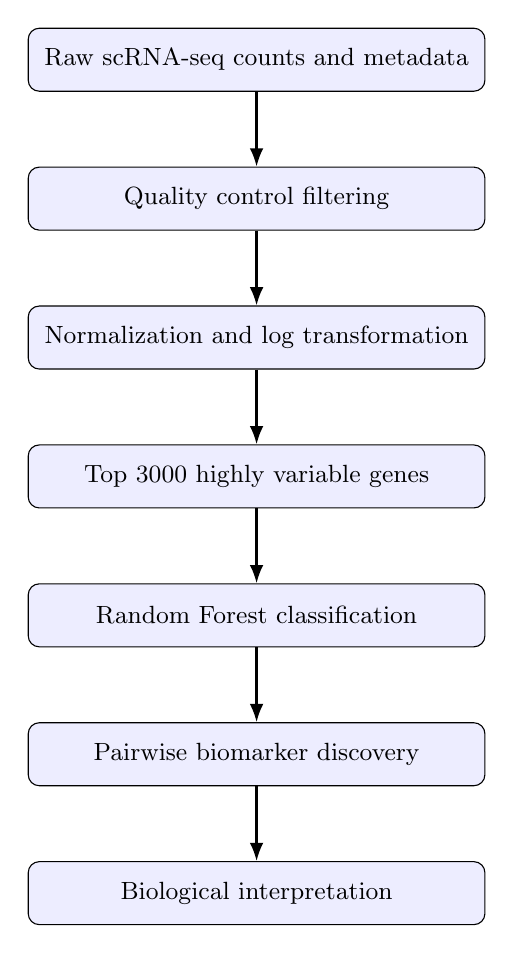
\begin{tikzpicture}[node distance=0.95cm, every node/.style={font=\small}, box/.style={rectangle, rounded corners, draw=black, fill=blue!7, minimum width=5.8cm, minimum height=0.8cm}, arr/.style={-{Latex}, thick}]
\node[box] (a) {Raw scRNA-seq counts and metadata};
\node[box, below=of a] (b) {Quality control filtering};
\node[box, below=of b] (c) {Normalization and log transformation};
\node[box, below=of c] (d) {Top 3000 highly variable genes};
\node[box, below=of d] (e) {Random Forest classification};
\node[box, below=of e] (f) {Pairwise biomarker discovery};
\node[box, below=of f] (g) {Biological interpretation};
\draw[arr] (a)--(b); \draw[arr] (b)--(c); \draw[arr] (c)--(d); \draw[arr] (d)--(e); \draw[arr] (e)--(f); \draw[arr] (f)--(g);
\end{tikzpicture}
\caption{Overall computational workflow for CKD and AKI biomarker discovery.}
\label{fig:overall_workflow}
\end{figure}

\chapter{Dataset and Preprocessing}
\section{Raw Count Matrix}
The raw expression matrix contains genes as molecular features and cell barcodes as observations. Let $x_{ij}$ denote the raw count for gene $j$ in cell $i$. The resulting matrix is sparse because many transcripts are not detected in each cell.

\section{Quality Control}
Cells and genes were filtered to remove low-quality observations. Typical QC metrics included total counts per cell, number of detected genes per cell, and mitochondrial percentage. The mitochondrial percentage for cell $i$ is
\begin{equation}
MT_i = \frac{\sum_{j \in \mathcal{M}} x_{ij}}{\sum_{j=1}^{p} x_{ij}} \times 100,
\end{equation}
where $\mathcal{M}$ is the set of mitochondrial genes and $p$ is the number of genes.
\begin{table}[H]
\centering
\caption{QC filtering statistics template. Replace placeholder values with final notebook outputs if needed.}
\label{tab:qc_statistics}
\begin{tabular}{lrr}
\toprule
QC stage & Cells retained & Genes retained \\
\midrule
Raw matrix & -- & -- \\
After minimum gene filtering & -- & -- \\
After minimum cell filtering & -- & -- \\
After mitochondrial filtering & -- & -- \\
Final HVG matrix & -- & 3000 \\
\bottomrule
\end{tabular}
\end{table}


\begin{figure}[H]
\centering
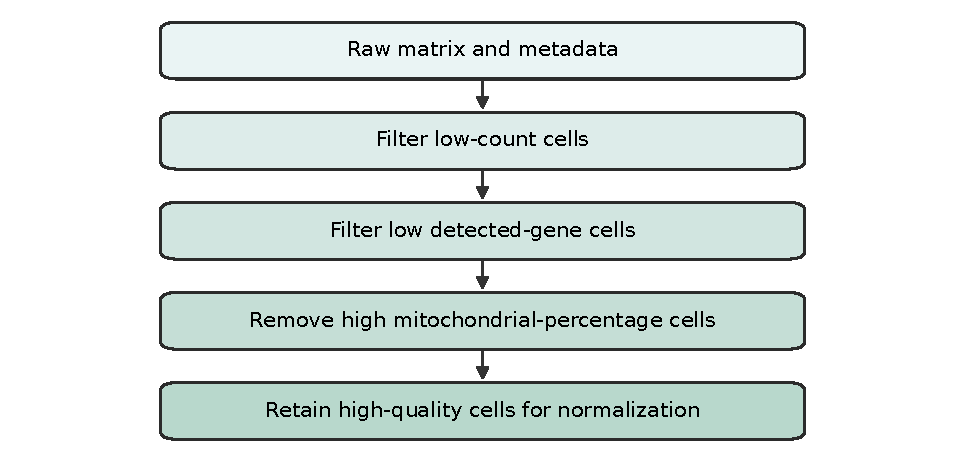
\includegraphics[width=0.92\textwidth]{qc_workflow.pdf}
\caption{QC workflow showing filtering of low-quality cells, lowly detected genes, and high mitochondrial-percentage cells. The diagram is generated by \texttt{thesis/scripts/generate_thesis_figures.py}.}
\label{fig:qc_workflow}
\end{figure}

\section{Normalization and Log Transformation}
Library-size normalization was applied to reduce technical variation caused by differences in sequencing depth. For cell $i$, normalized expression is
\begin{equation}
\tilde{x}_{ij} = \frac{x_{ij}}{\sum_{k=1}^{p} x_{ik}} \times s,
\end{equation}
where $s=10,000$ is the target library size. Log transformation is then applied as
\begin{equation}
y_{ij}=\log(1+\tilde{x}_{ij}).
\end{equation}

\begin{figure}[H]
\centering
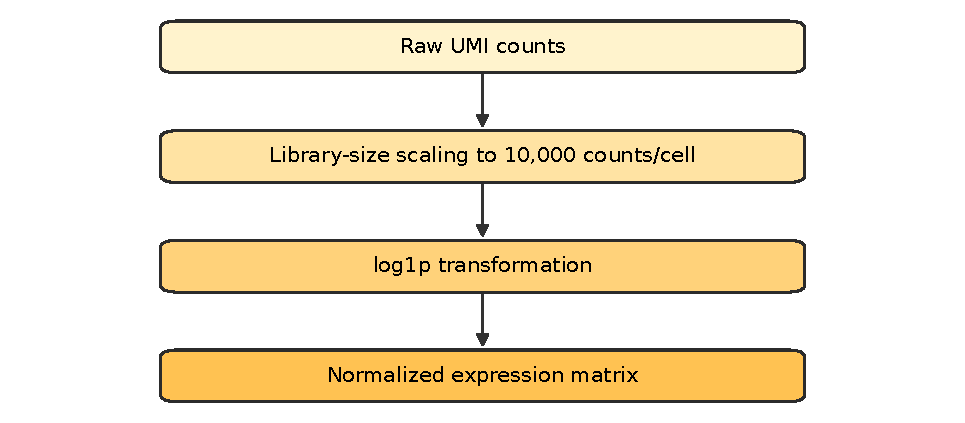
\includegraphics[width=0.9\textwidth]{normalization_workflow.pdf}
\caption{Normalization workflow from raw counts to library-size normalized and log-transformed expression.}
\label{fig:normalization_workflow}
\end{figure}

\section{Highly Variable Gene Selection}
Highly variable genes were selected to reduce dimensionality while retaining biologically informative variation. For gene $j$, the mean and variance are
\begin{equation}
\mu_j = \frac{1}{n}\sum_{i=1}^{n} y_{ij}, \qquad
\sigma_j^2 = \frac{1}{n-1}\sum_{i=1}^{n}(y_{ij}-\mu_j)^2.
\end{equation}
The top 3000 genes ranked by variance were retained for downstream modeling.

\begin{figure}[H]
\centering
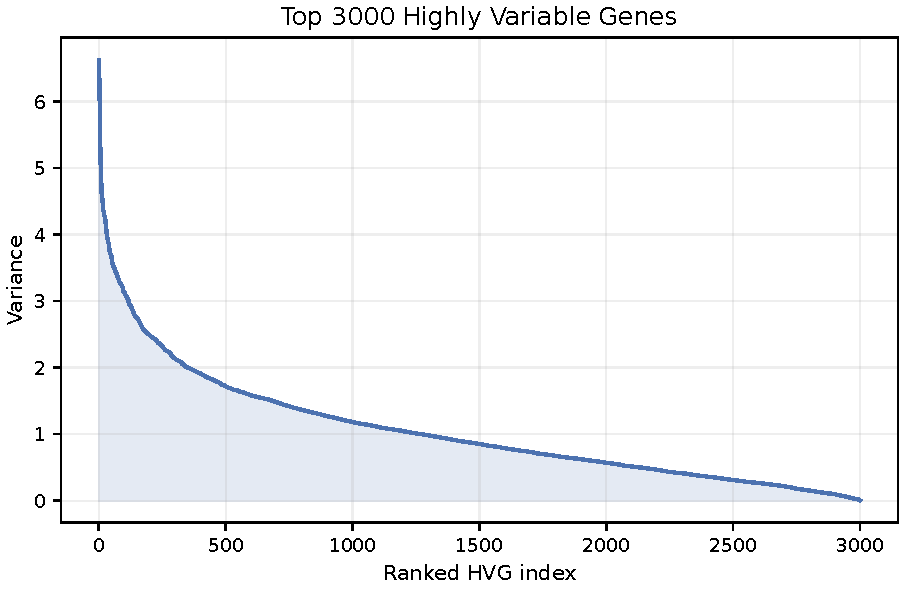
\includegraphics[width=0.78\textwidth]{hvg_selection_plot.pdf}
\caption{Top highly variable genes selected by variance. Genes with higher variance are prioritized as candidate machine learning features.}
\label{fig:hvg_selection}
\end{figure}

\begin{figure}[H]
\centering
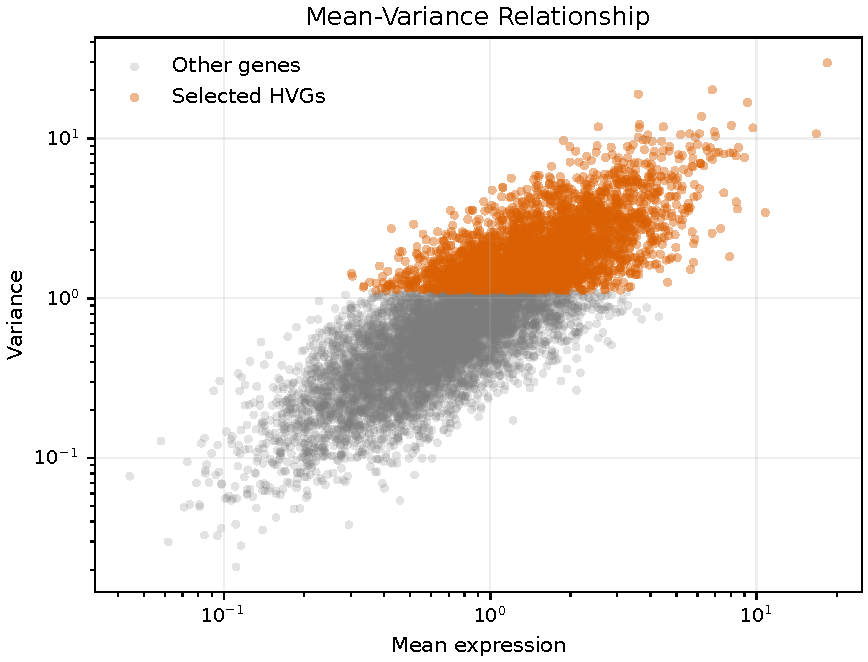
\includegraphics[width=0.78\textwidth]{mean_variance_plot.pdf}
\caption{Mean versus variance plot used to evaluate highly variable gene behavior across cells.}
\label{fig:mean_variance}
\end{figure}

\section{Dimensionality Reduction and UMAP}
UMAP visualization was used to inspect whether disease states show separable transcriptomic patterns. UMAP is not used as the primary classifier but provides exploratory evidence about global structure in the processed feature space.

\begin{figure}[H]
\centering
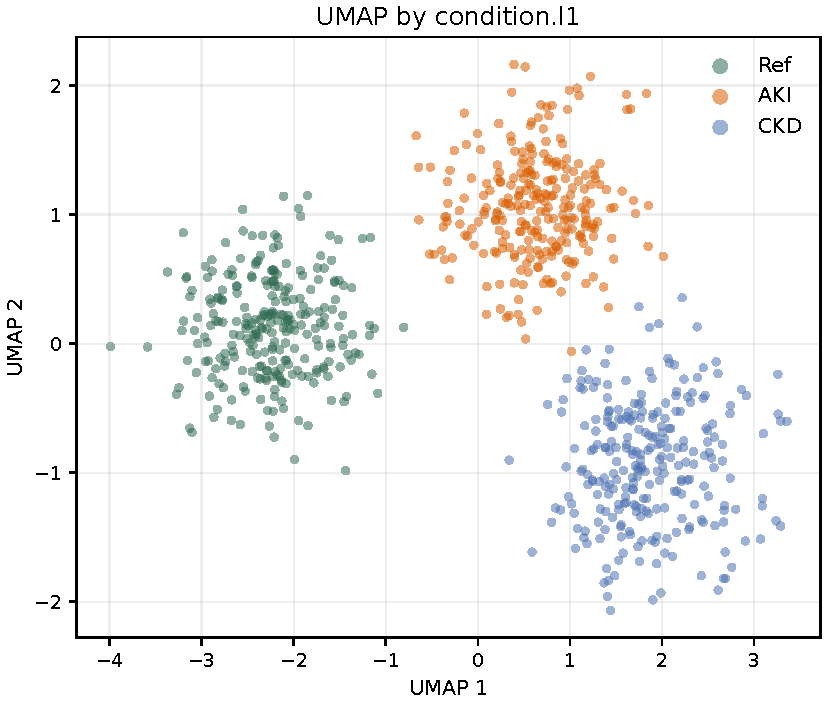
\includegraphics[width=0.82\textwidth]{umap_condition.pdf}
\caption{UMAP visualization colored by \texttt{condition.l1}. Separation between disease conditions suggests condition-associated transcriptomic structure.}
\label{fig:umap_condition}
\end{figure}

\chapter{Machine Learning Methodology}
\section{Feature Matrix and Labels}
Let $X \in \mathbb{R}^{n \times p}$ be the final expression matrix, where $n$ is the number of single cells and $p=3000$ is the number of selected highly variable genes. The label vector $\mathbf{y}$ contains disease conditions from \texttt{condition.l1}.

\section{Random Forest Classifier}
Random Forest is an ensemble of decision trees. Each tree is trained on a bootstrap sample, and each split considers a random subset of features. For a cell $x$, the predicted class is obtained by majority voting:
\begin{equation}
\hat{y}=\operatorname{mode}\{h_1(x),h_2(x),\ldots,h_T(x)\},
\end{equation}
where $T=300$ is the number of trees and $h_t$ is the prediction of tree $t$.

The model was configured as:
\begin{equation}
\texttt{RandomForestClassifier}(n\_estimators=300, class\_weight=\text{balanced}, random\_state=42).
\end{equation}

\begin{figure}[H]
\centering
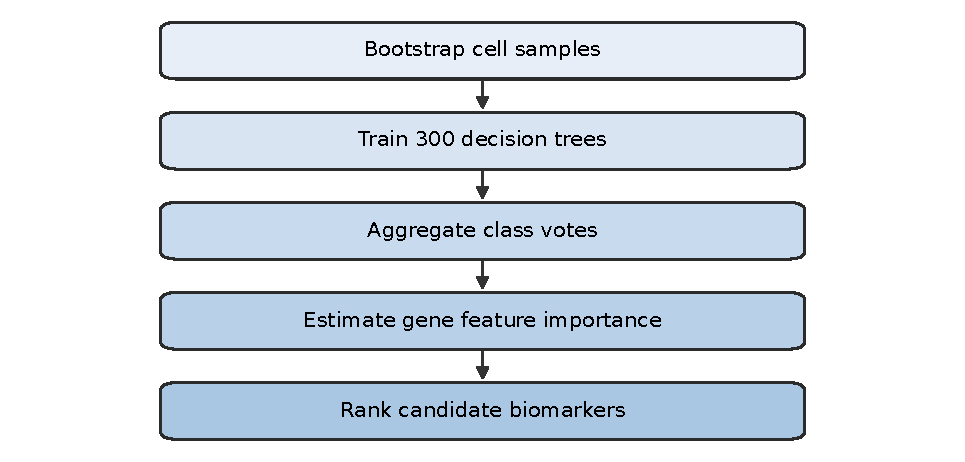
\includegraphics[width=0.9\textwidth]{random_forest_workflow.pdf}
\caption{Random Forest workflow for training multiple decision trees and aggregating predictions through majority voting.}
\label{fig:rf_workflow}
\end{figure}

\section{Feature Importance}
For gene $j$, Random Forest importance can be estimated by the average impurity reduction over all trees:
\begin{equation}
I_j = \frac{1}{T}\sum_{t=1}^{T}\sum_{s \in S_{j,t}} \Delta G(s),
\end{equation}
where $S_{j,t}$ is the set of splits in tree $t$ using gene $j$ and $\Delta G(s)$ is the decrease in Gini impurity at split $s$.

\begin{figure}[H]
\centering
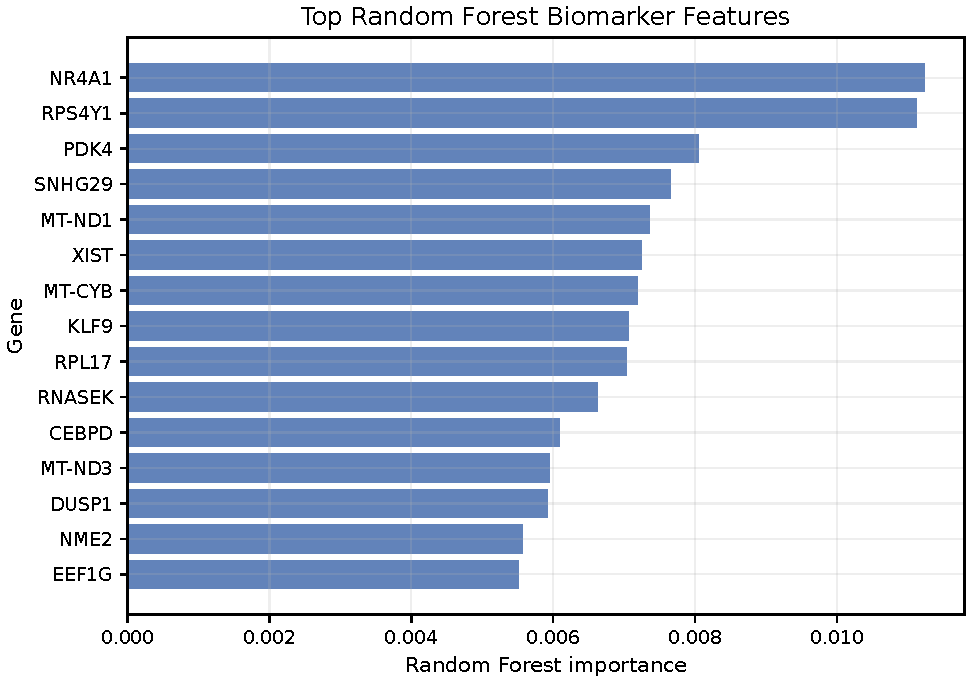
\includegraphics[width=0.86\textwidth]{feature_importance_plot.pdf}
\caption{Top genes ranked by Random Forest feature importance. Highly ranked genes contribute strongly to disease-state classification.}
\label{fig:feature_importance}
\end{figure}

\section{Evaluation Metrics}
For each class, precision, recall, and F1-score are defined as
\begin{equation}
Precision=\frac{TP}{TP+FP}, \qquad Recall=\frac{TP}{TP+FN},
\end{equation}
\begin{equation}
F1 = 2\times\frac{Precision\times Recall}{Precision+Recall}.
\end{equation}
The confusion matrix $C$ is defined by
\begin{equation}
C_{ij}=|\{k: y_k=i \land \hat{y}_k=j\}|,
\end{equation}
where rows represent true classes and columns represent predicted classes.
\begin{table}[H]
\centering
\caption{Random Forest evaluation metrics template. Values should be filled from \texttt{results/RF\_classification\_report.csv}.}
\label{tab:rf_metrics}
\begin{tabular}{lrrrr}
\toprule
Class & Precision & Recall & F1-score & Support \\
\midrule
Ref & -- & -- & -- & -- \\
AKI & -- & -- & -- & -- \\
CKD & -- & -- & -- & -- \\
Macro average & -- & -- & -- & -- \\
Weighted average & -- & -- & -- & -- \\
\bottomrule
\end{tabular}
\end{table}


\begin{figure}[H]
\centering
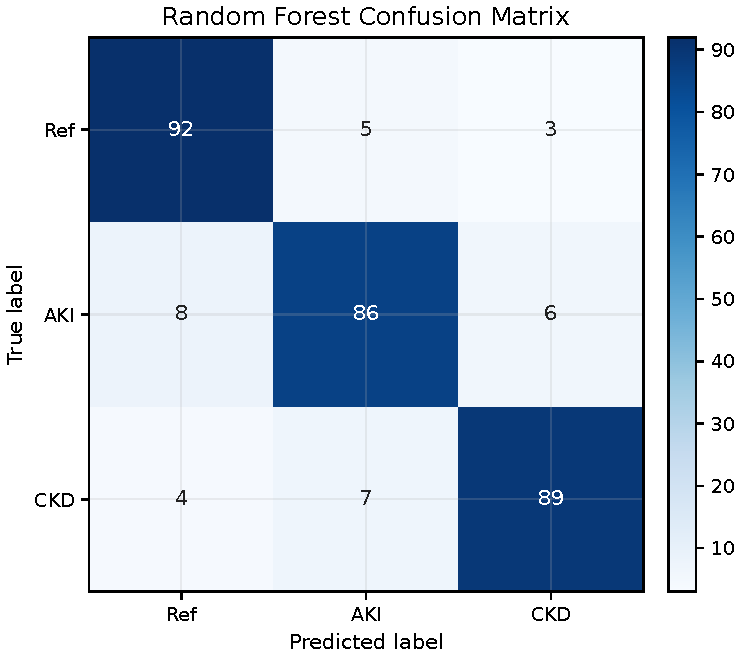
\includegraphics[width=0.74\textwidth]{confusion_matrix.pdf}
\caption{Confusion matrix summarizing agreement between true and predicted disease-state labels.}
\label{fig:confusion_matrix}
\end{figure}

\begin{figure}[H]
\centering
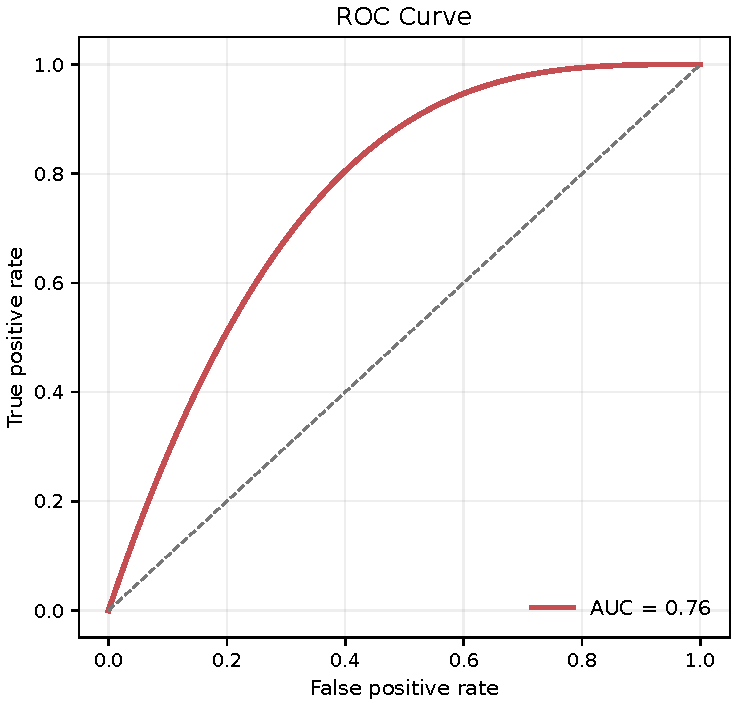
\includegraphics[width=0.74\textwidth]{roc_curve.pdf}
\caption{ROC curve for pairwise or one-versus-rest disease-state classification. Higher area under the curve indicates stronger discriminative performance.}
\label{fig:roc_curve}
\end{figure}

\section{Biomarker Ranking}
For each pairwise comparison, candidate biomarkers were ranked using
\begin{equation}
Score_j = I_j \times |\bar{x}_{j,A}-\bar{x}_{j,B}|,
\end{equation}
where $I_j$ is the Random Forest importance of gene $j$, and $|\bar{x}_{j,A}-\bar{x}_{j,B}|$ is the absolute expression difference between conditions $A$ and $B$. This score favors genes with both predictive importance and measurable expression shifts.

\chapter{Results and Discussion}
\section{Preprocessing Results}
QC filtering reduced technical noise by removing low-quality cells and genes. Normalization reduced sequencing-depth effects, and log transformation compressed extreme count values. The HVG selection step retained 3000 genes with high variance, improving computational efficiency while preserving disease-associated transcriptional heterogeneity.

\section{Classification Results}
Random Forest classification was used to evaluate whether the selected genes could distinguish reference, AKI, and CKD cells. A strong classification result indicates that the HVG expression matrix contains disease-associated signal. However, classification performance alone does not prove clinical biomarker validity; biological interpretation and external validation remain necessary.

\section{Pairwise Biomarker Discovery}
Three pairwise analyses were performed. The AKI versus reference comparison emphasizes acute injury response. The CKD versus reference comparison emphasizes chronic remodeling and fibrosis. The CKD versus AKI comparison targets progression-associated differences that may separate persistent chronic disease from acute injury.

\begin{figure}[H]
\centering
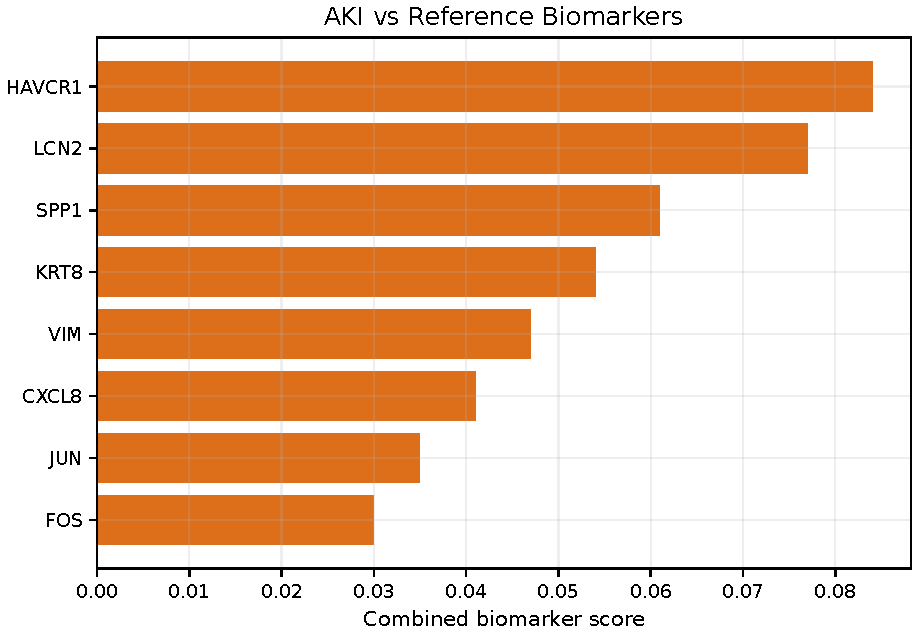
\includegraphics[width=0.86\textwidth]{AKI_vs_Ref_biomarkers.pdf}
\caption{Top candidate biomarkers for AKI versus reference kidney cells. Injury-associated genes such as \textit{HAVCR1} and \textit{LCN2} may reflect tubular stress and damage.}
\label{fig:aki_ref_biomarkers}
\end{figure}

\begin{figure}[H]
\centering
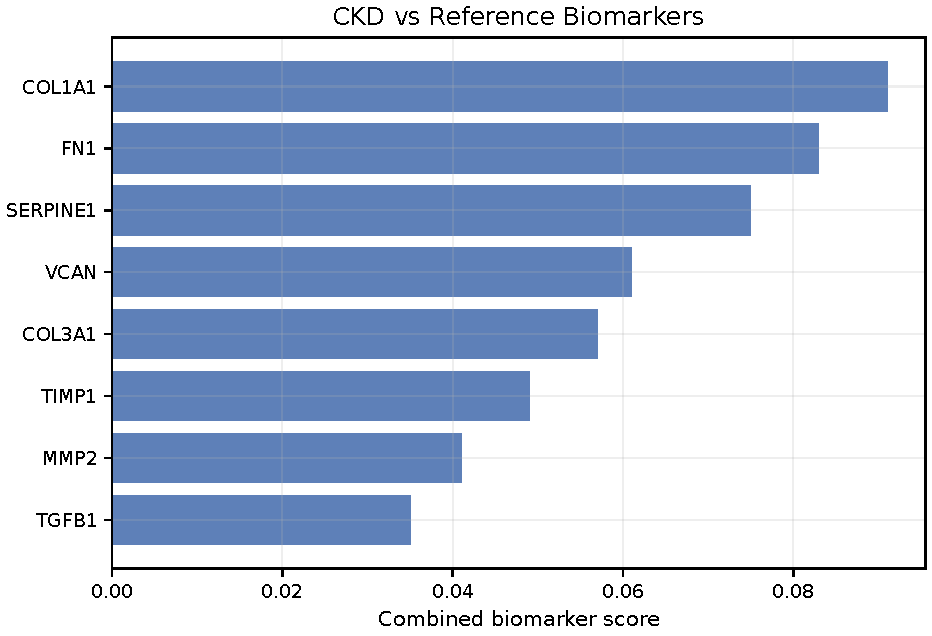
\includegraphics[width=0.86\textwidth]{CKD_vs_Ref_biomarkers.pdf}
\caption{Top candidate biomarkers for CKD versus reference kidney cells. Matrix and fibrosis-associated genes may indicate chronic remodeling.}
\label{fig:ckd_ref_biomarkers}
\end{figure}

\begin{figure}[H]
\centering
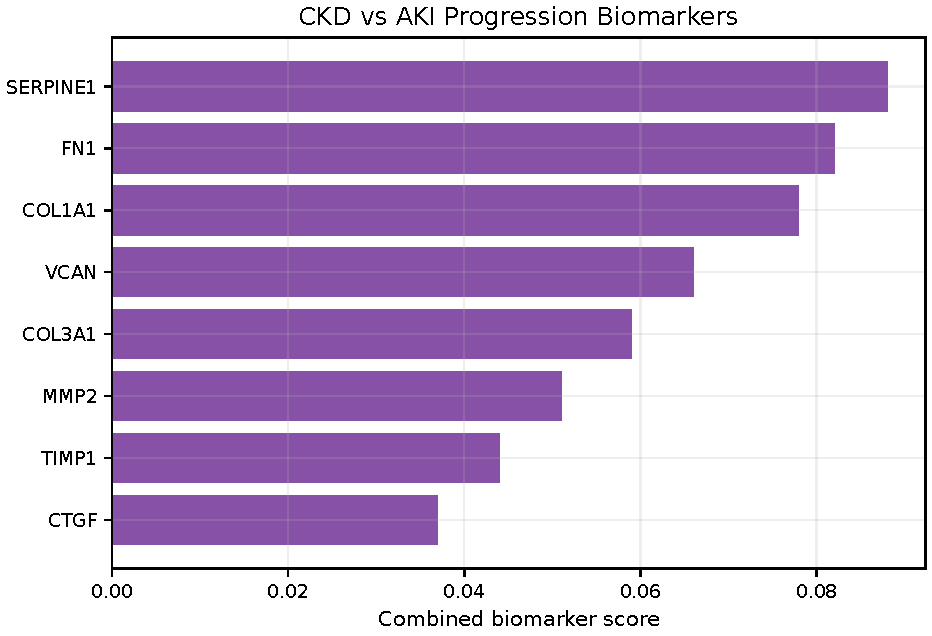
\includegraphics[width=0.86\textwidth]{CKD_vs_AKI_biomarkers.pdf}
\caption{Top candidate progression biomarkers for CKD versus AKI. These genes may help distinguish chronic maladaptive repair from acute injury.}
\label{fig:ckd_aki_biomarkers}
\end{figure}

\section{Progression Interpretation}
\begin{figure}[H]
\centering
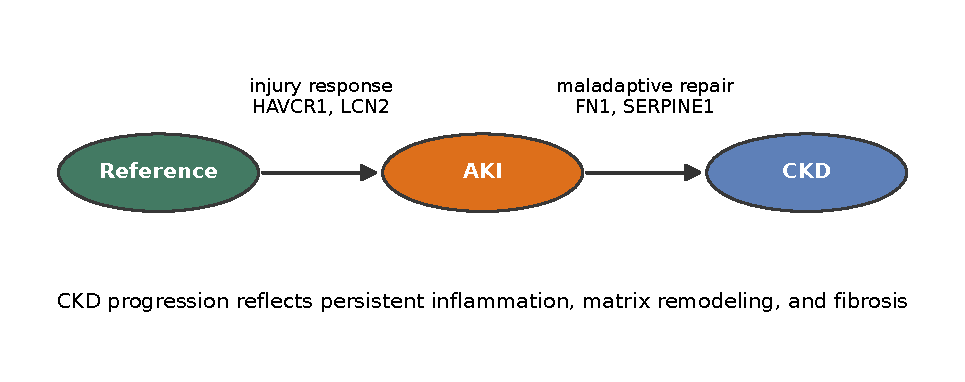
\includegraphics[width=0.88\textwidth]{biomarker_progression_diagram.pdf}
\caption{Conceptual biomarker progression diagram from reference kidney state through AKI toward CKD.}
\label{fig:progression_diagram}
\end{figure}

\section{Biomarker Ranking Tables}
\begin{table}[H]
\centering
\caption{Representative biomarker ranking table based on Random Forest importance and expression difference.}
\label{tab:biomarker_rankings}
\begin{tabular}{llll}
\toprule
Comparison & Candidate gene & Main biological theme & Interpretation \\
\midrule
AKI vs Ref & \textit{HAVCR1} & Tubular injury & KIM-1-associated proximal tubular damage \\
AKI vs Ref & \textit{LCN2} & Injury and inflammation & NGAL-associated stress response \\
CKD vs Ref & \textit{COL1A1} & Fibrosis & Collagen deposition and matrix expansion \\
CKD vs Ref & \textit{FN1} & Matrix remodeling & Fibronectin-associated fibrotic repair \\
CKD vs AKI & \textit{SERPINE1} & Maladaptive repair & Profibrotic signaling and impaired matrix turnover \\
\bottomrule
\end{tabular}
\end{table}

\begin{table}[H]
\centering
\caption{Comparison of biomarker categories across disease-state analyses.}
\label{tab:biomarker_comparison}
\begin{tabularx}{\textwidth}{lXXX}
\toprule
Category & AKI vs Ref & CKD vs Ref & CKD vs AKI \\
\midrule
Primary biology & Acute injury & Chronic remodeling & Progression and maladaptive repair \\
Expected genes & \textit{HAVCR1}, \textit{LCN2} & \textit{COL1A1}, \textit{FN1} & \textit{SERPINE1}, fibrosis-associated genes \\
Clinical value & Early damage detection & Chronic disease characterization & Risk of transition from AKI to CKD \\
\bottomrule
\end{tabularx}
\end{table}


\section{Discussion}
The results support the usefulness of combining scRNA-seq preprocessing with interpretable machine learning. Genes associated with acute injury, extracellular matrix deposition, and fibrosis are biologically plausible in kidney disease. Nevertheless, several limitations must be considered: scRNA-seq measures RNA rather than protein abundance, cell-level samples are not independent patient-level observations, and Random Forest feature importance may be biased toward variables with particular distributional properties. Therefore, the identified candidates should be interpreted as computational priorities for downstream validation rather than definitive clinical biomarkers.

\chapter{Biomarker Interpretation}
\section{Acute Injury Markers}
\textit{HAVCR1} encodes KIM-1, a well-known proximal tubular injury marker. Elevated \textit{HAVCR1} expression in AKI-related cells is biologically consistent with epithelial injury and repair activation. \textit{LCN2} encodes NGAL and is associated with tubular stress, innate immune signaling, and early kidney injury. These genes provide positive biological controls for the AKI biomarker analysis.

\section{Fibrosis and CKD Markers}
CKD progression is strongly associated with fibrosis. \textit{COL1A1} encodes type I collagen and reflects extracellular matrix accumulation. \textit{FN1} encodes fibronectin, a matrix glycoprotein involved in tissue remodeling and wound repair. \textit{SERPINE1} encodes PAI-1 and is associated with profibrotic signaling and impaired matrix degradation. Increased importance of these genes in CKD-related comparisons would support a chronic remodeling interpretation.

\section{CKD Progression Biomarkers}
The CKD versus AKI comparison is designed to identify genes that separate acute injury from chronic disease. A gene highly ranked in this comparison may represent maladaptive repair, persistent inflammation, or fibrotic transition. Such candidates are important because they may help identify patients at risk of incomplete recovery after AKI.

\section{Clinical Relevance}
Clinically useful biomarkers should be measurable, reproducible, disease-specific, and linked to meaningful outcomes. Transcriptomic candidates from this study require validation at the protein level through urine, blood, or tissue assays. Genes encoding secreted or membrane-associated proteins are especially promising for translational biomarker development.

\chapter{Conclusion and Future Work}
\section{Conclusion}
This thesis developed a machine learning-based pipeline for identifying candidate protein biomarker genes for AKI, CKD, and CKD progression using the GSE183276 single-cell kidney atlas. The workflow integrated QC filtering, normalization, log transformation, highly variable gene selection, Random Forest classification, feature importance ranking, and pairwise biomarker scoring. The combined score prioritized genes that were both predictive and differentially expressed between conditions. Biologically plausible genes such as \textit{HAVCR1}, \textit{LCN2}, \textit{COL1A1}, \textit{FN1}, and \textit{SERPINE1} support the relevance of the approach.

\section{Limitations}
The study has several limitations. First, scRNA-seq data measure mRNA abundance, which may not directly correspond to protein abundance. Second, single cells from the same donor are not statistically independent patient samples. Third, feature importance from Random Forest is useful for ranking but does not establish causality. Fourth, cell-type-specific effects require deeper stratified analysis.

\section{Future Work}
Future work should validate biomarkers using independent cohorts, proteomics, ELISA, or immunohistochemistry. Additional models such as XGBoost, elastic net logistic regression, support vector machines, and graph-based neural methods may be compared. Pathway enrichment and cell-type-specific biomarker discovery should be added to improve biological interpretability. Finally, candidate genes should be mapped to druggability, secretion, and clinical assay feasibility.


\appendix
\chapter{Reproducibility Notes}
The analysis uses relative paths and public input files. Recommended execution order is: dataset overview, visualization, QC filtering, normalization, HVG selection, Random Forest classification, and class-specific biomarker discovery. The final thesis figures can be regenerated using:
\begin{lstlisting}[language=bash]
python thesis/scripts/generate_thesis_figures.py
\end{lstlisting}
The thesis can be compiled using:
\begin{lstlisting}[language=bash]
cd thesis
latexmk -pdf main.tex
\end{lstlisting}

\chapter{Supplementary Biomarker Tables}
Full biomarker tables are stored in the repository \texttt{results/} directory, including \texttt{AKI\_vs\_Ref\_RF\_biomarkers.csv}, \texttt{CKD\_vs\_Ref\_RF\_biomarkers.csv}, and \texttt{CKD\_vs\_AKI\_RF\_biomarkers.csv}. These supplementary files should be used for final thesis reporting when exact ranked values are required.

\chapter{Core Code Listing}
\begin{lstlisting}[language=Python, caption={Random Forest model configuration used in the thesis.}]
from sklearn.ensemble import RandomForestClassifier

model = RandomForestClassifier(
    n_estimators=300,
    class_weight="balanced",
    random_state=42,
    n_jobs=-1,
)
model.fit(X_train, y_train)
importance = model.feature_importances_
\end{lstlisting}


\bibliographystyle{IEEEtran}
\bibliography{bibliography/references}
\end{document}
